\documentclass[12pt]{article}
\usepackage[utf8]{inputenc}
\newcommand\preamble{
    \usepackage[italian]{babel}
    \usepackage{geometry}
    \usepackage{amsmath}
    \usepackage{amssymb}
    \usepackage{graphicx}
    \usepackage{ulem}
    \usepackage[dvipsnames]{xcolor}

    \geometry{margin=2cm}
    \let\olditemize\itemize
    \renewcommand\itemize{\olditemize\setlength\itemsep{0em}}
    \graphicspath{{../Immagini/}}

    \author{Lorenzo Vaccarecci}
}
\preamble

\title{Ottimizzazione Fisica (Parte 2)}
\date{3 Maggio 2024}

\begin{document}
\maketitle
\section{Operatori Fisici}
\textcolor{red}{Sono implementazioni specifiche di un operatore
logico (ad esempio del join), basate su un certo
algoritmo di realizzazione}.\\ Esistono diversi algoritmi di realizzazione per ogni operatore logico. Algoritmi diversi possono utilizzare diverse informazioni contenute a livello fisico.\\
\textcolor{red}{La possibilità di usare un certo operatore fisico e quindi generare un certo piano fisico dipendono dallo schema fisico esistente (org primaria e indici).}\\
Operatori fisici:
\begin{itemize}
    \item Accesso alle relazioni di base
    \item Operazioni di relazione
    \item Operazioni di Join
\end{itemize}
\subsection{Accesso alle relazioni di base}
Il nostro piano sarà un albero (PQP). Le foglie sono le relazioni, l'accesso alle foglie avviene tramite \textcolor{red}{cammini di accesso}.
\subsubsection{Cammini di accesso}
Descrive come accedere al file dei dati di una relazione.
\begin{itemize}
    \item \textcolor{red}{Scansione sequenziale}
    \item \textcolor{red}{Indice più una condizione di selezione (Predicato di ricerca)}: utilizzabile solo se esiste una condizione di selezione che può essere eseguita usando l'indice
\end{itemize}
\textbf{Esempio:}
\begin{verbatim}
    SELECT * FROM R WHERE R.A=5
\end{verbatim}
\Tree [ .$\sigma_{A=5}$ R ]
\\Può essere implementato in due modi:
\begin{itemize}
    \item Accesso sequenziale
    \item alla scansione sequenziale si aggiunge $(I_{A}(R),A=5)$
\end{itemize}
Ogni cammino di accesso diventa un nodo foglia.
\begin{verbatim}
    SEQ SCAN R Filter (A=5)
    INDEX SCAN (I_{A}(R),A=5)
\end{verbatim}
\textbf{Esempio:}
\begin{verbatim}
    SELECT * FROM R WHERE R.A <> 5
\end{verbatim}
Non posso usare l'indice, quindi ho solo la scansione sequenziale. Perchè io devo trovare tutte le tuple che soddisfano la condizione, ma non posso sapere a priori quali sono.
\textbf{Esempio:}
\begin{verbatim}
    SELECT * FROM R WHERE R.A=5 AND R.B=6
\end{verbatim}
\Tree [ .$\sigma_{A=5 AND B=6}$ R ]
\begin{verbatim}
    SEQ SCAN R Filter (A=5 AND B=6)
    INDEX SCAN (I_{A}(R),A=5) Filter (B=6)
    INDEX SCAN (I_{B}(R),B=6) Filter (A=5)
\end{verbatim}
\textcolor{Cyan}{\textit{Dopo avere acceduto la relazione, è
necessario filtrare (scartare) le tuple che non
soddisfano l’altro congiunto}}.
Per accedere una singola relazione, \textcolor{Cyan}{può anche essere scelto più di
un cammino di accesso}, combinando poi i risultati con un ulteriore
operatore fisico.
\textbf{Esempio:}
\begin{verbatim}
    SELECT * FROM R WHERE R.A=5 AND R.B=6
    INDEX SCAN (I_{A}(R),A=5)
    INDEX SCAN (I_{B}(R),B=6)
\end{verbatim}
E poi i risultati delle due scan vengono intersecati.
\begin{center}
    \Tree [ .INTERSECTION [ .INDEX\_SCAN(I_{A}(R),A=5) ] [ .INDEX\_SCAN(I_{B}(R),B=6) ] ]
\end{center}
Con l'\textbf{OR} è simile ma si usa l'unione.
\subsubsection{Costi}
\begin{itemize}
    \item \textcolor{red}{Costo di accesso}: numero di pagine di blocco lette
    \item \textcolor{red}{Costo di selezione}: tipo di indice e numero di tuple che soddisfano il predicato
\end{itemize}
Costo totale = (costo di determinare i riferimenti ai dati che soddisfano la condizione, in organizzazione secondaria (1 per hash, $h(\log n)$ per albero)) + (costo per accedere ai
corrispondenti blocchi dei
dati in organizzazione
primaria, la clusterizzazione influisce).
\begin{itemize}
    \item Indice ordinato clusterizzato: \textcolor{Cyan}{Ogni blocco dati viene letto al più una volta}
    \item Indice ordinato non clusterizzato: \textcolor{Cyan}{Un blocco può essere acceduto più volte}
    \item Indice non ordinato clusterizzato: \textcolor{Cyan}{Un blocco può essere acceduto più volte}, i puntatori ai blocchi vengono ordinati. (Operatore BITMAP)
\end{itemize}
\subsection{Operazioni di relazione}
\subsubsection{Selezione}
\question{Cosa succede se eseguo una selezione su un risultato intermedio?}
La selezione può essere implementata solo in modo sequenziale perchè \important{non è possibile utilizzare un indice su un risultato intermedio.}
\subsubsection{Join}
E' un'operazione costosa: richiede $T(R)\cdot T(S)$ confronti (dove $T(R)$ e $T(S)$ sono il numero di tuple delle due relazioni). Per evitare tutti i possibili confronti:
\begin{itemize}
    \item \important{Nested Loop Join}: Si accede ad una tupla di $R$ (outer relation) e si confronta con ogni tupla di $S$ (inner relation). L'ordine corrisponde all'ordine delle tuple della relazione esterna. Costi: $B(R) + T(R) \cdot B(S)$. \important{Conviene considerare come relazione outer la relazione più grande}.
    \item \important{Index Nested Join}: Come il nested loop join, ma si utilizza un indice su $S$ per accedere alle tuple e si usa solo se esiste l'indice. Costi: $B(R)+T(R) \cdot$costo di accesso a $S$.
    \item \important{Merge Join}: \textcolor{Cyan}{ applicabile quando le relazioni in input sono ordinate rispetto all’attributo di join}. \important{L’algoritmo sfrutta il fatto che entrambi gli input sono
    ordinati rispetto all’attributo di join}. Prima avviene l'ordinamento delle relazioni, poi si scansionano le relazioni in parallelo e si fanno i confronti tupla per tupla.
    \item \important{Hash Join}: applico la funzione hash alle tuple delle due relazioni e le metto in un bucket. Se due tuple hanno lo stesso hash, vengono messe nello stesso bucket. Si calcola il join tra i bucket. \important{Sicuramente due tuple in due bucket diversi non possono essere in join}, se sono nello stesso bucket \textbf{potrebbero} essere in join.
\end{itemize}
$B(\cdot)$ è il numero di blocchi letti.
\begin{center}
    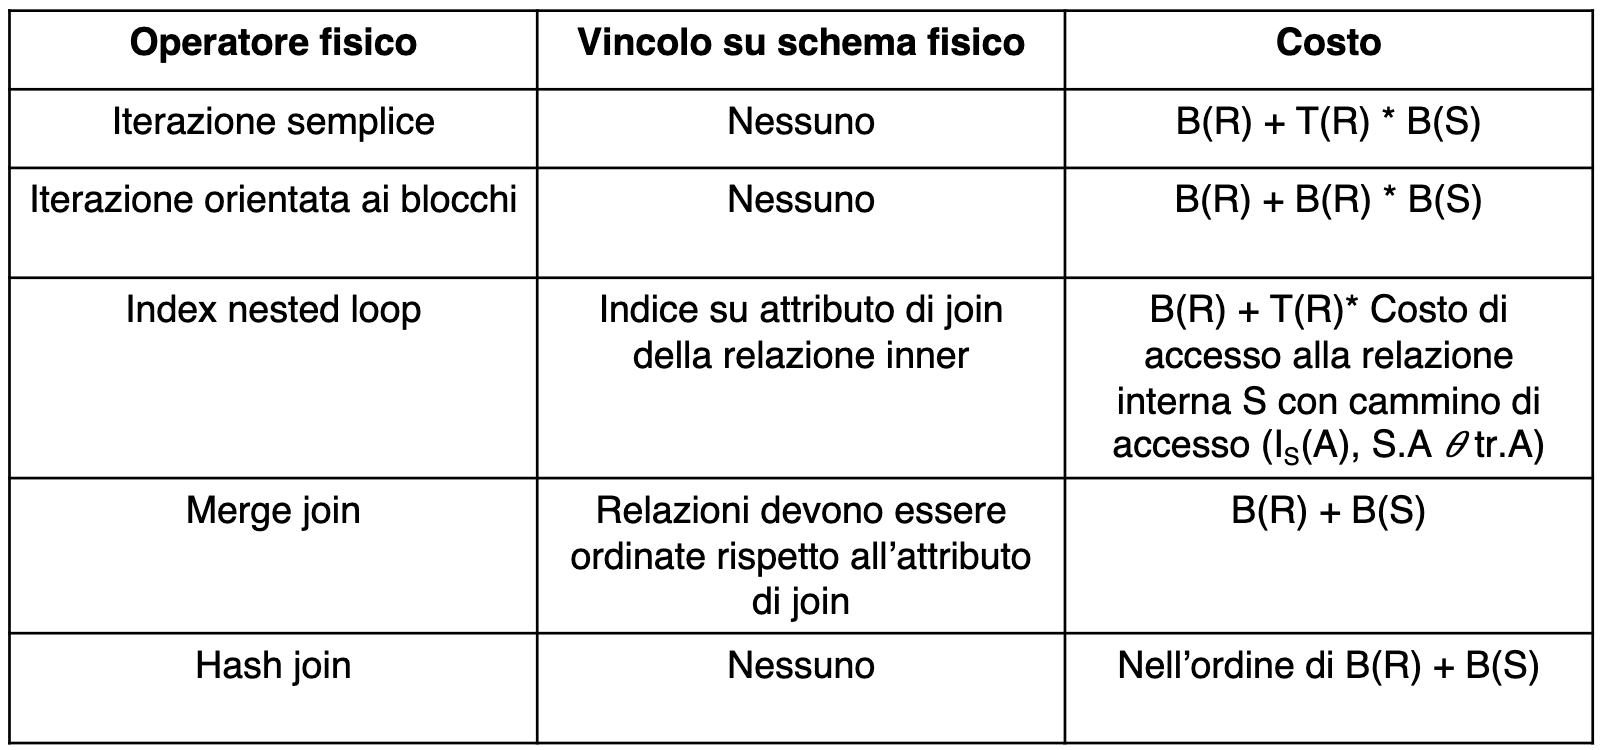
\includegraphics[scale=0.5]{opfisici.png}
\end{center}
\subsection{Condizioni più generali}
\begin{itemize}
    \item \important{Uguaglianza su più di un attributo}
    \item \important{Theta-join con disuguaglianza}
\end{itemize}
\end{document}